% #############################################
	\section{Methods} \label{sec:system}
% #############################################


The proposed system consists of several stages, namely: time series segmentation and feature extraction from  FHR signals; similarity calculation with NCD, for which the combination of similarity matrices can provide with further advantage; and choice of a suitable classification algorithm for the final purpose of hypoxia detection. The theoretical basis and design criteria of these stages are described below.



%#############################################################################################
\subsection{Time Series Segmentation and Feature Extraction}  \label{subsec:feat:extraction}
%#############################################################################################

%%we summarize the time series segmentation criteria to be considered at the design stage, we present several sets of features with statistical and physiological meaning, and we summarize a feature selection procedure used for determining the sufficient subset of features.
%
%%\textsc{\myorange{The following paragraphs are ordered in subsubsections, but just for sake of clarity. This will be removed in future versions.}}
%
%%{\it Segmentation.} 
%%\subsubsection{Segmentation}
%
%{\it Time series segmentation.} We decided to consider the analysis of the FHR signal in one-hour windows, in order to determine the accuracy that can be attained at three, two, and one hours before delivery. This will show whether hypoxia signs can be detected before these time milestones, hence allowing to make decisions as quick as possible on stressed foetuses. Second, we consider all the signal present from 4 hours to 1 hour before delivery, aiming to mimic the comparison of one fetus in labor (when we do not know the remaining labor time). % within our database of labeled records of fetuses. All the patients with FHR signal recorded in part of an interval are considered in the analysis of this interval.  
%Finally, we also analyzed the  FHR signals by dividing them into a set of short sliding windows, which is a usual practice in heart rate signals analysis~\cite{Signorini:2003ee}.
%
%
%%\subsubsection{Feature Extraction}
%
%{\it Feature extraction.}  Feature extraction techniques aim to gather specific parameters from a signal which can be easier to analyze than the signal samples itself. The use of the raw data is theoretically supported by the data processing inequality, which states that signal processing cannot increase the  information content~\cite{cover91_information_theory}. However, information loss cause by feature extraction is preferable to raw data analysis as it simplifies later classification or estimation. In this work, we consider several types of features to be extracted from the fetal signals. On the one hand, Heart Rate Variability (HRV) parameters are commonly used for analyzing heart signals in different applications~\cite{Malik:96}, and they require their own preprocessing stage. On the other hand, statistical moments can be considered as general use parameters for characterizing signals in general. Though statistical moments discard the temporal structure of a time signal, they are known to be robust to signal loses and easy to compute.
%
%{\it FHR features from HRV conventional analysis.} FHR conventional analysis is often performed using time domain and frequency domain indices computed on 5 minutes segments. For linear HRV analysis, a preprocessing algorithm is applied to the raw signal to deal with noise and artifacts related to the fetal and maternal movements. Beats lower than 60 beats per minute (bpm), and beat-to-beat differences higher than 25 bpm, are identified by the preprocessing algorithm as noise or artifacts. Those beats labeled as low quality (see below) are also identified as artifacts~\cite{Goncalves:2006ga,Signorini:2003ee}. Then, every beat identified as an artifact is removed and replaced using linear interpolation. 
%Segments with more than five consecutive samples (beats) identified as artifacts or with more than 5\% artifacts are discarded for the analysis. Finally, FHR signals are subsequently resampled at  2 Hz (following~\cite{Goncalves:2006ga}), keeping only the odd samples.
%
%Let $s[n]$, for $n = 1,\ldots,N$,  be the set of values of FHR signal, also denoted by $\bs$ in vector form. The following time domain indices~\cite{Magenes:2000jb} can be computed:
%\begin{equation}
%\mfhr = \bar{s} = \frac{1}{N}\sum^{N}_{n = 1}s[n]
%\end{equation}
%\begin{equation}
%stdFHR = \sqrt{\frac{1}{N-1}\sum^{N}_{n = 1}(s[n]-\bar{s})^{2}}
%\end{equation}
%\begin{equation}
%LTI = \text{IQR}\left(\left\{\sqrt{s^2[n]+s^2[n+1]},\ 1\le n \le N - 1\right\}\right)
%\end{equation}
%\begin{equation}
%STV = \frac{1}{24M}\sum^{24M}_{n = 1} \left| sm[n+1]-sm[n] \right|
%\end{equation}
%where IQR denotes the inter-quartile range, $M$ is the number of the minutes in the segment under analysis, $sm[n]$ is the value of the signal $s[n]$ taken each $2.5$ seconds (i.e., once each five samples), and \emph{std} means  standard deviation.
%
%Frequency domain indices are often computed by using nonparametric spectral estimation based on Welch periodogram, with a \emph{Hanning} window, on 256 samples segments, and with 50\% overlapping~\cite{Bernardes:2008in}. The mean and the linear trend are usually subtracted before calculating the periodogram. FHR variability is usually assessed by computing the total power in different frequency bands, which are~\cite{Signorini:2003ee}: Very Low Frequency, $P_{VLF}$ in $(0,0.03)\ Hz$; Low Frequency, $P_{LF}$ in $(0.03,0.15)\ Hz$; Movement Frequency, $P_{MF}$ in  $(0.15,0.5 Hz)$; and High Frequency, $P_{HF}$ in $(0.5,1 Hz)$. VLF  is usually related with thermo-regulatory processes, and LF and HF are associated with the autonomic nervous system (ANS) regulation~\cite{Malik:1996vo}. MF is typical of FHR, but it is not present in HRV in adults, and is related with the fetal movements and maternal breathing. Total power ($P_T$) and the ratio $P_{LF}/(P_{MF}+P_{HF})$ are also computed as frequency domain indices.


%{\it Features from Statistical Moments.} Moments are simple descriptors of the shape of the distribution of a random set of values~\cite{fisher37:_momen_cumul_specif_distr}. Their use has been useful in many signal processing problems~\cite{Shi2005,Soliman1992}, and they are robust to signal losses, as they can be  computed on the known signal samples while ignoring the unknown time periods. The  $k^{th}$-order raw moment, and the corresponding central moments, are defined as:
%\begin{eqnarray}  \label{eq:raw:moments}
%  M_k(\bs) & = & \frac{1}{N}\sum_{n=1}^N s[n]^k \\ \label{eq:central:moments}
%  \mu_k(\bs) & = & \frac{1}{N}\sum_{n=1}^N (s[n]-M_1(\bs))^k .
%\end{eqnarray}
%
%
%%\subsubsection{Feature Selection}
%{\it Feature Selection.} Feature selection techniques aim for the selection of the variables subset providing with all the information about a task with the minimum redundancy among  them~\cite{guyon03:_introd_variab_featur_selec}. This  provides three benefits for the resulting models: improved generalization, better interpretability, and shorter training and execution times. Among these techniques,  wrapper methods build a model for each candidate set and select the model with the best performance on a validation set. We propose to use here two wrapper methods:
%\begin{itemize}
%\item  Automatic threshold selection (ATS) retrieves  those features with individual training accuracy above a threshold, which is automatically selected in the training set to maximize the classification accuracy.
%\item Forward selection (FS) iteratively adds to the included feature subset the non-included feature providing with the best accuracy in the training set. The number of features is automatically selected in the training set as the minimum number that reaches the maximum accuracy. In order to control overfitting, each feature candidate set can be evaluated by 2-fold cross-validation on the training sample.
%\end{itemize}





%%##########################################################
%\subsection{NCD and Similarity in Time Signals}
%##########################################################
%[Podemos comenzar con una motivación cualitativa para NCD. Si no, para el que no conozca esto entramos muy a saco.]


%%{\it Fundamentals of NCD Algorithm.} 
%A simple approach to classification is to assign to the test object the label of the closest or the most similar object in a training dataset. The accuracy of this approach depends on the goodness of the distance measure for representing differences and similarities among the objects to be classified. The best measure would  match all the common patterns among the objects, at the same time that it would detect their differences. Given an object (in our case, signal $\bs$), similarity learning~\cite{Pekalska2002} uses as features the similarities ($\{d(\bs,\bt_i)\}$ for $i=1,\ldots,N_T$)  to a labelled training set $\{\bt_i\}$ of $N_T$ objects. Then, a machine learning classifier can be readily trained by using these features. 
%
%We choose here a general similarity measure that is based on the common information among the signals, and which can handle both linear and nonlinear relations among them. Kolmogorov Complexity $K(\bs)$ of a signal $\bs$ is the length of the shortest binary program that produces $\bs$ on an universal Turing machine~\cite{kolmogorov1965three,Li2004}. Note that $K(\bs)$ can be seen as the information of the signal (or the information needed to generate it); $K(\bs|\bt)$ is the length of the shortest program  to produce $\bs$ if $\bt$ is given as an input; and $K(\bs,\bt)$ is the length of the shortest program that generates $\bs$, $\bt$, and allows to separate them. Up to an additive  constant independent of  $\bs$, $\bt$, it can be proven~\cite{Li2004} that
%\begin{equation}
%K(\bt,\bs)=K(\bt) +K(\bs|\bt)  = K(\bs) + K(\bt|\bs)\;.
%\end{equation}
%
%The information distance between two signals is a similarity measure~\cite{bennett1998} that can be defined as
%\begin{equation} 
%ID(\bt,\bs)=  \max\{K(\bs|\bt), K(\bt|\bs)\} \;,
%\end{equation}
%It has two problems for its practical use, namely,  Kolmogorov Complexity is not computable and we need a distance suitable for comparing signals of different sizes. 
%
%NCD is a similarity measure for signals~\cite{Li2004,Cilibrasi2005}. Given two signals $\bs_i,\bs_j$, the NCD$(\bs_i,\bs_j)$ is defined as
%\begin{equation}  \label{eq:ncd}
%  \text{NCD}(\bs_i,\bs_j)=\frac{C(\bs_i,\bs_j)-\min\{C(\bs_i),C(\bs_j)\}}{\max\{C(\bs_i),C(\bs_j)\}} \; ,
%\end{equation}
%where $C(\cdot)$ is the compression length in bits given by the selected compressor $C$ ($C(\bs_i)$ and $C(\bs_i,\bs_j)$ are  the  number of bits needed to compress $\bs_i$ and the concatenation of $\bs_i$ and $\bs_j$), respectively. Note that $C$ provides a computable approximation to the Kolmogorov Complexity. This normalized measure has a simple interpretation, in the sense that the lower its value, the more similar the signals. In other words,  they share more information and fewer bits are required to compress both signals together. The normalization term in the denominator of~\eqref{eq:ncd} enables the comparison among signals of different sizes. Note also that NCD values range from zero to slightly above one.
%
%As far as NCD is just an approximation to the Kolmogorov Complexity, its performance can be improved by simplifying the compressor work. In other words, we can apply NCD to series of features computed in  sliding-windows instead of applying it to the raw signals, with the aim of extracting the patterns that NCD is not able to resolve in the raw signals. 
%
%%\myorange{Still not clear this combination of similarity features: it combines the features, the output of differente experts (then this should go in the classifcation engine subsection). May be a deep reading is needed.}
%%{\it Combination of similarity features.} %[Podemos comentar cómo se puede trabajar con varias matrices de similaridad, y su pertinencia para utilizarlas con distintos tipos de características combinadas, como es el caso de este trabajo.]
%
%Another possible approach for improving the performance of NCD is to combine several sets of similarity features, which can be generated by applying the same measure to different parts of the signal or by different measure types. The following are easy to use strategies for similarity combination:
%\begin{itemize}
%\item {\it Concatenation.} All the similarities to the training points are concatenated to form a single vector of features. 
%\item {\it Sum.} When the similarities are of the same type, they share the same scale and therefore the ones referred to the same training example can be combined in a soft way with a simple sum.  Even different types of similarities can be combined by suitable scaling. This approach is sensitive to outliers.
%\item {\it Decision combination.} A decision is taken according to each similarity. Then, all the decisions are combined into a global decision output. In this work, we propose to combine the decisions by simple voting.
%\end{itemize}
%
%%##########################################################
%\subsection{Classification Engine}
%%##########################################################
%
%{\it Classification Algorithms.} 
%On the one hand, the detailed physical model that generates the FHR records is complex and mostly unknown. On the other hand, we have some set of available observations, but we  have no enough data to estimate  the conditional densities of the classes for diagnosis. Hence,  we propose to use a non-parametric machine learning approach for classification, and for this purpose we consider two approaches, namely, $k$ Nearest Neighbors ($k$-NN), which is easy to combine with similarity measures, and Support Vector Machines (SVM), a state-of-the-art and advantaged classifier in a number of applications. 
%
%In a binary classification problem, we are given a collection of labelled samples $\{\bx_i,y_i\}$ $i=1,\ldots,N_T$, where $\bx_i \in \mathbb{R}^D$ and $y_i \in \{-1,1\}$.
%The $k$-NN  algorithm~\cite{Duda2000} selects the label for a test sample as the mode of the labels of the $k$ training instances that are nearest to it (its $k$ nearest neighbours). In case of tie, the decision can be taken at random or with the label of the closest neighbor. The distance between samples is defined by a similarity measure, which is usually the euclidean distance, but in our case it will be given by NCD instead. The asymptotic error of this simple classifier is bounded by twice the Bayes error, which is the minimum  attainable error~\cite{Cover1967}. In general, NCD similarity is not symmetric, and $\text{NCD}(\bs_i,\bs_j) \ne \text{NCD}(\bs_j,\bs_i)$. Therefore, to obtain the similarity among $\bs_i$ and $\bs_j$,  we scrutinized two flavors of similarity: type \emph{min} using the minimum similarity, $\min\{\text{NCD}(\bs_i,\bs_j), \text{NCD}(\bs_j,\bs_i)\}$, and type \emph{mean} using the mean, $0.5 (\text{NCD}(\bs_i,\bs_j) + \text{NCD}(\bs_j,\bs_i))$. 
%
%SVM are powerful learning machines that can be easily trained and have been successfully used in many applications~\cite{cortes95:_suppor_vector_networ,scholkopf01_learning_with_kernels}. The trained classifier for binary classification is the solution of the following convex optimization problem:
%\begin{equation}\label{SVM1}
%\min_{\bw,b,\xi_i} \frac{1}{2}||\bw||^2+C\sum_i\xi_i
%\end{equation}
%subject to:
%\begin{align}\label{rest_SVM1}
%y_i(\bw^\top \bphi(\bx_{i})+b)&\geq 1-\xi_i\\
%\xi_i&\geq 0\label{rest_SVM2}
%\end{align}
%where $\bw$ is the classifier solution and it can be written as a combination of the training samples, i.e., $\bw=\sum_i \beta_i \bphi(\bx_i)$. The objective function has two terms, the former is a regularization term that penalizes rough solutions, and the later penalizes the classification errors, both being balanced by parameter $C$.  Positive slack variable $\xi_i$  accounts for the margin error of sample $i$, which allows for getting solutions in non-separable problems; $(\cdot)^\top$ is the transpose operator; $\bphi()$ is a function  projecting $\bx_i$ into a possibly higher dimensional space where the linear classification is done, which allows for non-linear classification functions in the original space $\mathbb{R}^D$;  and $b$ is  a bias term. The prediction for a new sample $\bx^*$ is $y^*=\sign (\bw^\top \bphi(\bx^*)+b) = \sign( \sum_i k(\bx^*,\bx_i) + b)$, where $k(\bx_i,\bx_j)$ is a kernel that computes $\bphi(\bx_i)^\top \bphi(\bx_j)$ without explicitly evaluating $\bphi(\cdot)$. We consider here two kernel functions, namely, the linear kernel $k(\bx_i,\bx_j)= \bx_i^\top \bx_j$, and the radial basis function kernel  $k(\bx_i,\bx_j)= \exp{\left(-\frac{||\bx_i- \bx_j||^2}{2\sigma^2}\right)}$, where $\sigma$ defines the kernel width. Finally, Equation~\eqref{rest_SVM1} shows that SVMs enforce a margin for classification, i.e., the label times the output of the classifier should be greater that 1, allowing for margin errors by paying a penalty. Not all the margin errors are classification errors, but only those ones with $\xi_i \geq 1$.
%
%{\it Performance Evaluation.}  In some applications  where the labelled instances are scarce, a usual approach is to estimate the performance of the classification on unseen test cases by cross-validation~\cite{Duda2000}. In this paper, the accuracy of the different alternatives has been estimated by using leave-one-out (LOO) cross-validation.  We choose the almost unbiased LOO accuracy estimation, even at the cost of its high variance, because we have a extremely low number of examples in our dataset.
%, and accuracy estimation takes advantage of the largest training data length. % Following best machine learning practices, parameter and feature selections (if used) are performed only on the training data for each cross-validation step. 
%\myorange{Take-home message to be transformed into a more digestible form}
The procedure can be summarized as follows:
%\begin{algorithmic}
%\ForAll{$i$}
%\State $\bX_T= \bX \backslash \bx_i$
%\State $\bY_T= \bY \backslash y_i$
%\State $\text{Feature selection: } FS=g(\bX_T,\bY_T)$ 
%\State $\text{Classifier training: } f=h(\bX_T,\bY_T,FS)$
%\State $\text{Prediction: } \hat{y}_i=f (\bx_i,FS) $
%\EndFor
%\State $\text{Performance evaluation: } p=L(\bY,\hat{\bY})$
%\end{algorithmic}
%where $\bX = \{\bx_i\}$, $\bY=\{y_i\}$, $\hat{\bY}=\{\hat{y}_i\}$, $i=1,\ldots,N_T$; ``$\backslash$'' means set subtraction (i.e., $\bX \backslash \bx_i=\{\bx_1, \bx_2, \ldots, \bx_{i-1}, \bx_{i+1},\ldots,\bx_{N_T}\}$), $g,h$  are  feature selection and classifier training algorithms, respectively; $FS$ are the selected features; and $L$ is the 0--1 loss function.




%##########################################################
% Section data description
%##########################################################
\section{Data description}\label{sec:data}
\myblue{FHR  records\footnote{Data  is available from the website: http://sites.google.com/site/hufahypoxia.} were acquired with a Philips cardiotocograph for a total of 32 recordings, 15 controls and 17 cases. A case was declared whether: 1) the PH of the umbilical artery was $\leq$ 7.05; or 2) the APGAR score was $\leq$ 7 at 5 minutes after delivery  and a reanimation type III or greater was required. The institutional Medical Ethics Review Board approved the use of this data.}

\myblue{Records, see Figure~\ref{fig:RAWFHR} for an example, have considerable variability both in start/ending times and  pauses as labor duration vary. In addition, the cardiotocograph may be disconnected at any time for a number of reasons. Also, the signal is lost sometimes as the fetus and mother move.  The  cardiotocograph provides three signal qualities (lost, medium and high). We decided to consider the window between 4 to 1 hours before birth for our analysis, even though not all patients have signal along all this window, e.g. nine patients even start being monitored after 4 hours to delivery (8 cases) or they are removed the cardiotocograph before  1 hour to delivery (one case). When a patient has no signal in the entire interval analyzed in a experiment, it was excluded (see below).}

%\textcolor{declared-color}{text}
\begin{figure}[tp]
\centering%
\subfigure[hypoxic]{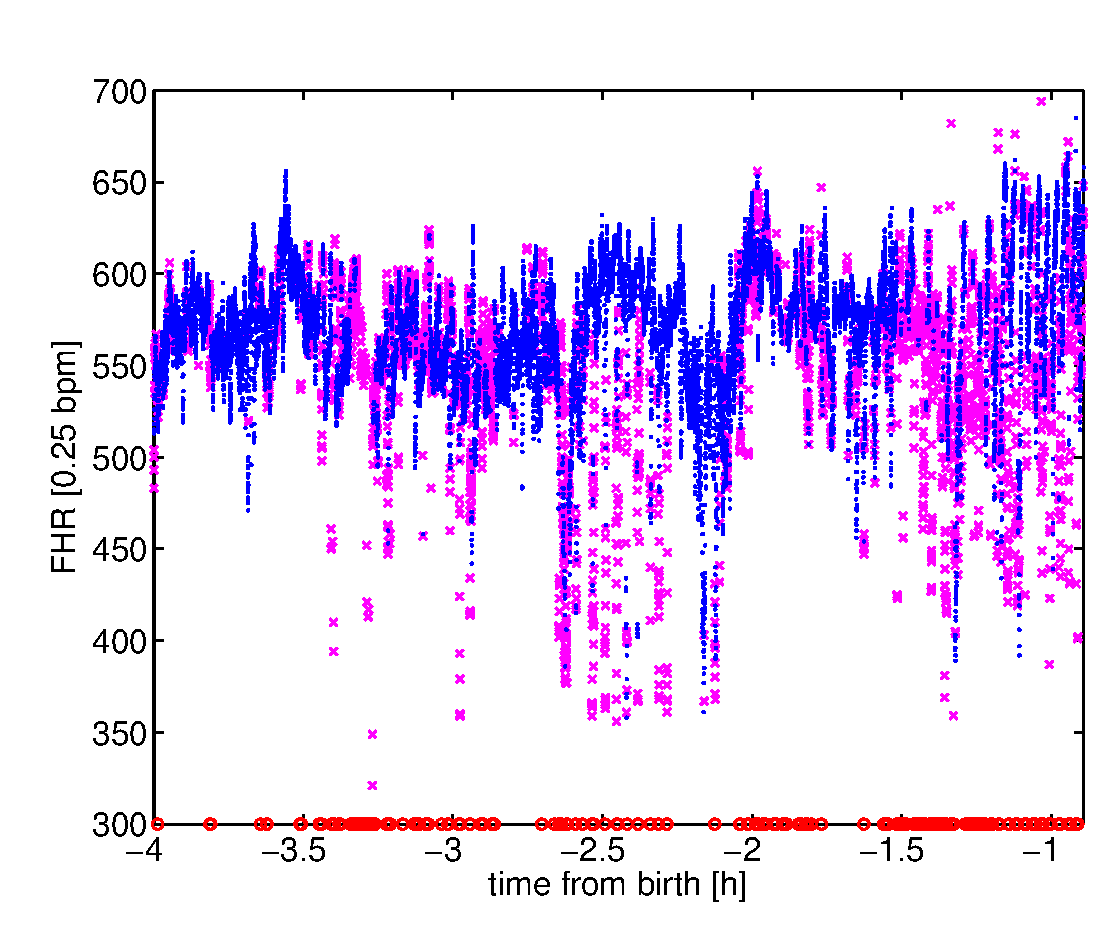
\includegraphics[width=0.9\linewidth]{./figs/caso}}\\%
\subfigure[control]{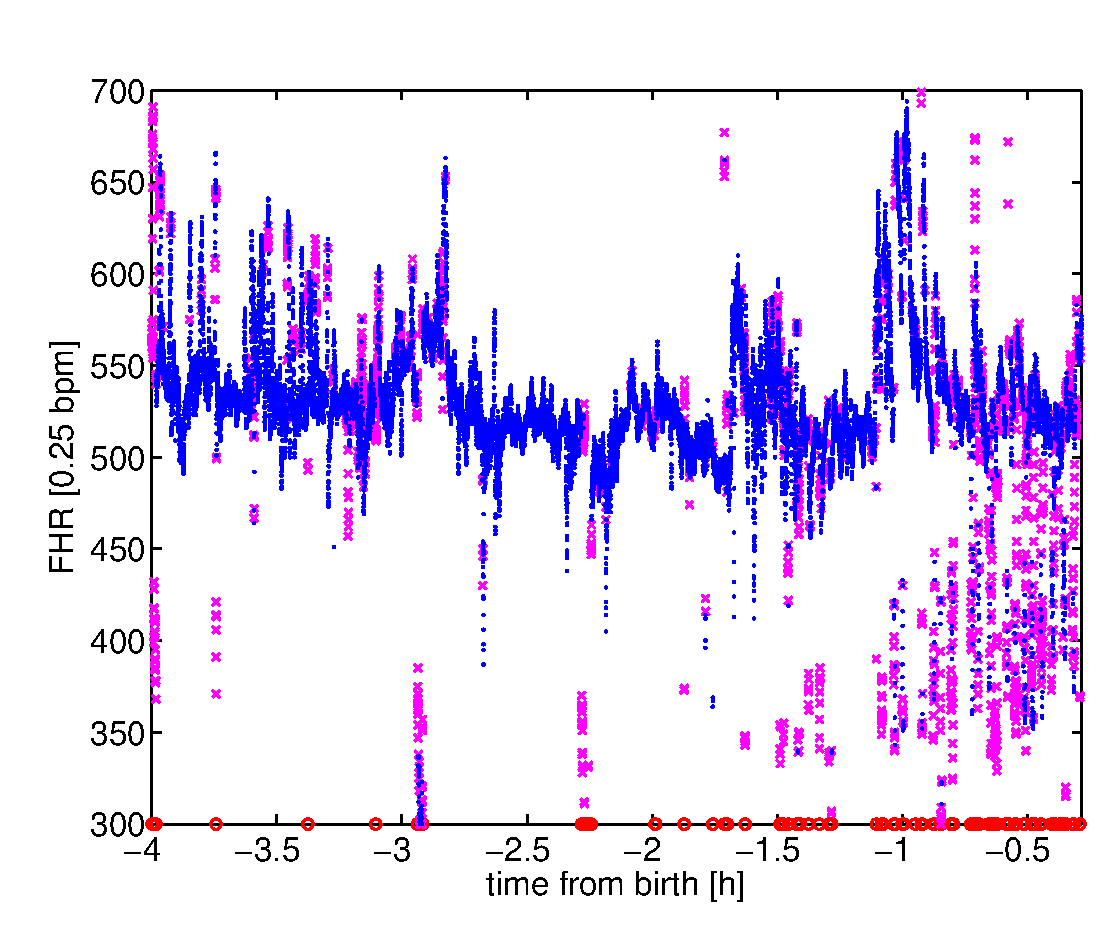
\includegraphics[width=0.9\linewidth]{./figs/control}}
\caption{FHR for (a) a hypoxic and (b) a control patient. Signal qualities are 9.9\% lost, 19.2\% medium and 70.9\% high for (a) ; and 1.8\% lost, 9.8\% medium and 88.3\% high for (b).  Signal qualities  high, medium and lost  are respectively represented by the markers: ``\textcolor{blue}{$\cdot$}'', ``\textcolor{magenta}{x}'' and ``\textcolor{red}{o}''.}
\label{fig:RAWFHR}
\end{figure}
%##########################################################
% Section data description
%##########################################################


